\def\theme{TP - Frises et pavages}
\def\date{20/11/2023}
\def\authors{
    PESIN - CADOT - COURTIN
}

\def\tikzScale{0.5cm}
\def\side{3}
\def\figShift{(0, 0)}
\def\fig{(0,0) -- (\side,0) -- (\side,\side) -- (0,\side) -- cycle}

\newcommand{\drawSquare}[2]{
    \draw[line width= 0.25mm, #1, shift= #2] \fig;
}

A l'aide du logiciel \textbf{Scratch} :
\begin{enumerate}

    \item Tracer un carré de 20 pas de côté.\\
    \begin{center}
        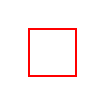
\begin{tikzpicture}[x=\tikzScale, y=\tikzScale]
            \drawSquare{red}{\figShift};
            \drawPoint{A}{0}{\side}{\figShift};
            \drawPoint{B}{\side}{\side}{\figShift};
            \drawPoint{C}{\side}{0}{\figShift};
            \drawPoint{D}{0}{0}{\figShift};
        \end{tikzpicture}
    \end{center}

    \item Tracer l'image de ce carré par la translation de A vers B.
    q
    \item Tracer une frise de 10 carrés comme ci-dessous:
    \begin{center}
        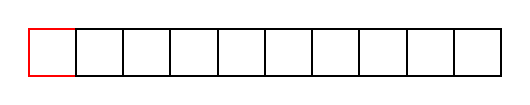
\begin{tikzpicture}[x=\tikzScale, y=\tikzScale]
            \drawSquare{red}{\figShift};
            \foreach \n in {1,...,9}
                \drawSquare{black}{{(\n * \side,0)}};
        \end{tikzpicture}
    \end{center}
\end{enumerate}

\hint{}{
    \begin{itemize}
        \item Scratch le chat peut se retrouver bloqué sur les côtés du cadres.\\
        Pensez à le faire toujours apparaître à un endroit bien choisi de la zone de jeu lorsque vous appuyez sur le drapeau vert.
        \item Pensez à bien utiliser à des boucles.
    \end{itemize} 
}

\vspace*{0.5cm}

\textbf{Bonus:}

\begin{enumerate}
    \item Rendre la taille du carré et le nombre de motifs modifiable par deux variables.
    \item Tracer un pavage de 10 par 10 comme ci-dessous:
    \def\side{1.2}
    \begin{center}
        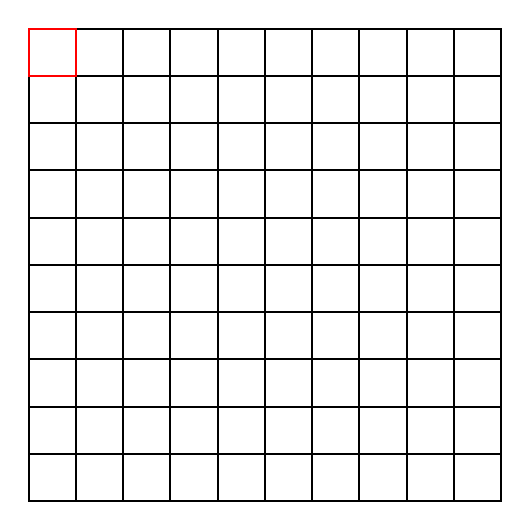
\begin{tikzpicture}[x=\tikzScale, y=\tikzScale]
            \foreach \n in {0,...,9}
                \foreach \m in {0,...,9}
                    \drawSquare{black}{{(\n * \side, -\m * \side)}};
                \drawSquare{red}{\figShift};
        \end{tikzpicture}
    \end{center}
    
\end{enumerate}